\chapter{Methodology}

\section{Uni-variate Model}
\subsection{Exponential Smoothing}

\subsubsection{Theory}
A forecasting technique for univariate time series data is exponential smoothing. With this strategy, forecasts are weighted averages of historical observations, with the weights of older observations decreasing exponentially. The study can now include model data with trends and seasonal components thanks to various forms of exponential smoothing.

In the 1950s, statisticians first developed exponential smoothing. Since then, it has had enormous success among analysts as a rapid method of producing precise projections in a variety of disciplines, particularly in industry. Additionally, it is utilised in signal processing to filter high-frequency noise and smooth signals.

The simplest form of an exponential smoothing formula is given by:
$$ s_t = \alpha x_t+(1 – \alpha)s_{t-1}= s_{t-1}+ \alpha(x_t – s_{t-1}) $$

Here,

$s_t$ = smoothed statistic, it is the simple weighted average of current observation $x_t$

$s_{t-1}$ = previous smoothed statistic

$\alpha$ = smoothing factor of data; $0 < \alpha < 1$

$t$ = time period

\subsubsection{Python Script} 
\begin{lstlisting}[language=Python]
from statsmodels.tsa.holtwinters import ExponentialSmoothing
# prepare data
data = df6['inflation-cpi'].iloc[:-12].dropna()
# create class
model = ExponentialSmoothing(data,trend='add', seasonal='add',seasonal_periods=12)
# fit model
model_fit = model.fit()
predic = model_fit.forecast(12)

#model summary
model_fit.summary()

# Residual Plot
model_fit.resid.plot()

#Ploting Fitted and Actual values
plt.plot(df6['tmp'][:-12],df6['inflation-cpi'].iloc[:-12],color="gray")
plt.plot(df6['tmp'][:-12],model_fit.fittedvalues,color="red")
plt.show()

# RMSE value for Model
from sklearn.metrics import mean_squared_error
rms = mean_squared_error(df6['inflation-cpi'].iloc[-12:], predic, squared=False)
rms1 = mean_squared_error(dfnew['inflation-cpi'].iloc[:-12], model_fit.fittedvalues, squared=False)
print("RMSE of Fitted: ",rms1)
print("RMSE of out of Sample forecast: ",rms)

\end{lstlisting}

\subsubsection{Model Summary} 
\begin{figure}[H]
    \centering
    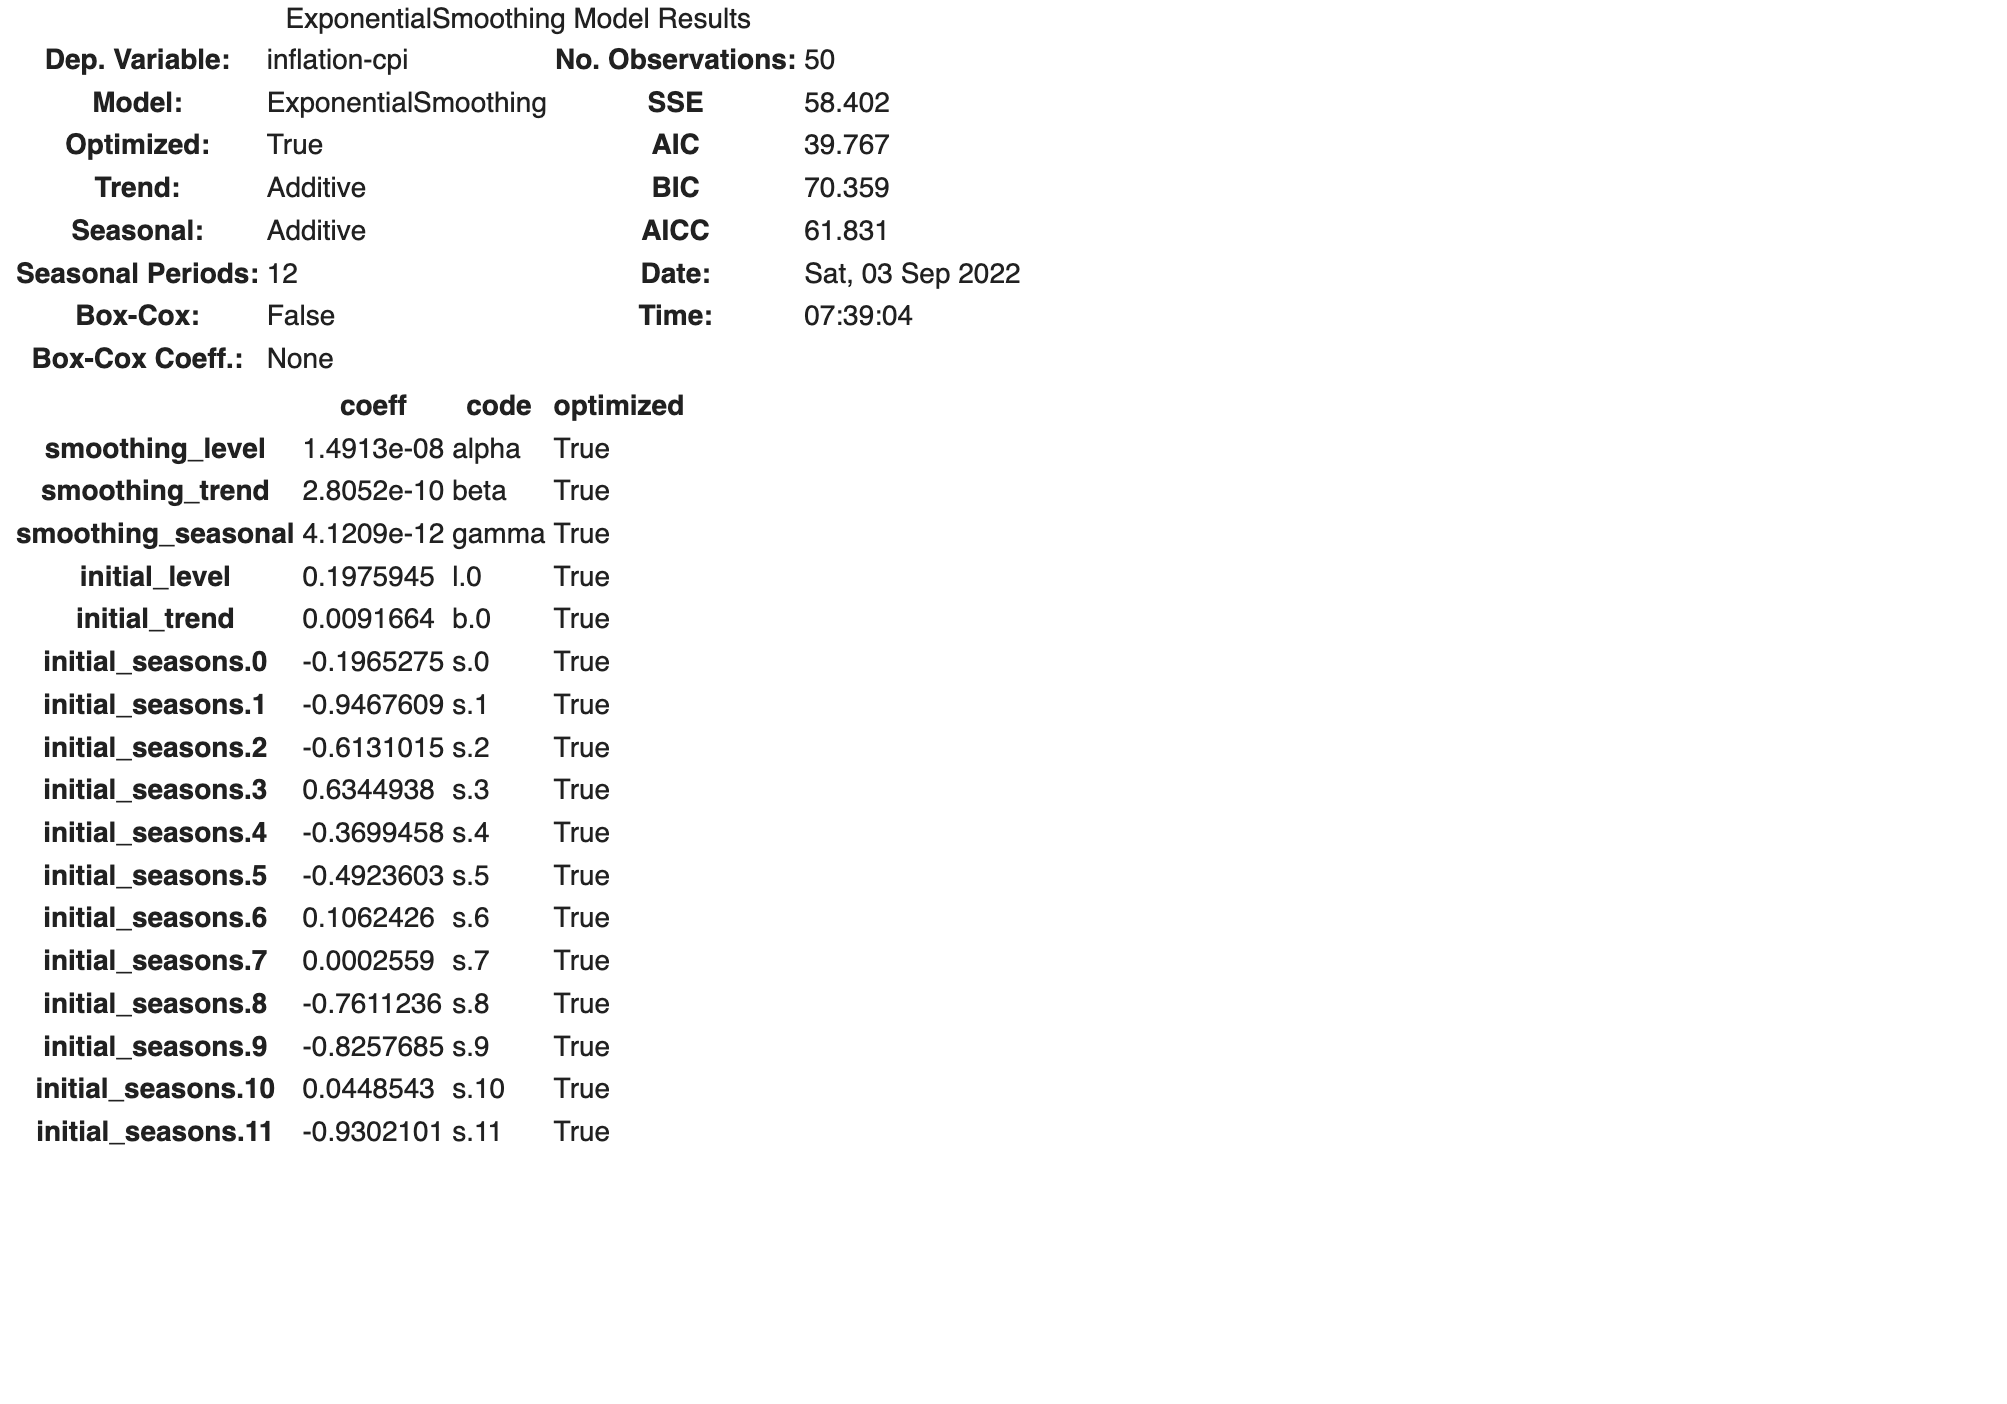
\includegraphics[width=0.7\textwidth]{Images/EXP.png}
    \caption{Summary}
    \label{fig1}
\end{figure}

\begin{figure}[H]
    \centering
    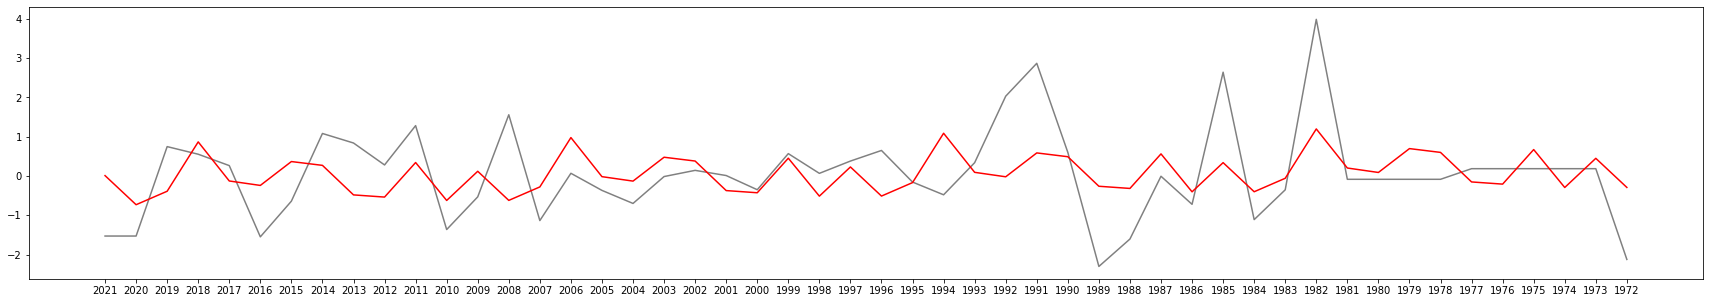
\includegraphics[width=0.7\textwidth]{Images/EXP_P.png}
    \caption{Output Plot}
    \label{fig1}
\end{figure}




Root Mean Squared Error:  2.161697017697318


\subsection{Auto-regressive Moving Average (ARMA)}
\subsubsection{Theory}
\begin{figure}[H]
    \centering
    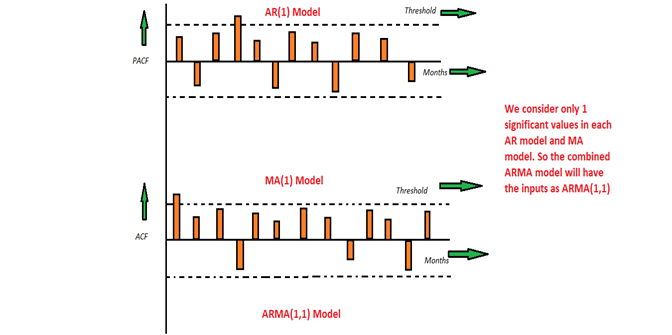
\includegraphics[width=0.7\textwidth]{Images/arma_model.png}
    \caption{ARMA}
    \label{fig1}
\end{figure}

The AR and MA models were combined to create this model. In this model, residuals and the effects of earlier lags are taken into account when predicting future values of the time series. Here, $\beta$ stands for the AR model's coefficients and $\alpha$ for the MA model's coefficients.

$$Y_t = \beta_1* y_{t-1} + \alpha_1* \varepsilon_{t-1} + \beta_2* y_{t-2} + \alpha_2 * \varepsilon_{t-2} + \beta_3 * y_{t-3} + \alpha_3 * \varepsilon_{t-3} +………… + \beta_k * y_{t-k} + \alpha_k * \varepsilon_{t-k}$$



Consider the above graphs, where the MA and AR values are shown along with their corresponding significant values. Let's assume that we only take into account 1 significant value each from the AR model and the MA model. The ARMA model will therefore be created by adding the data from the previous two models, and it will have the ARMA order (1,1)


\subsubsection{Python Script} 
\begin{lstlisting}[language=Python]
# ARMA model
data = df6['inflation-cpi'].dropna().iloc[:-12]
# MA model
model = ARIMA(data, order=(2,0,1))
model_fit = model.fit()
predic = model_fit.forecast(12)
model_fit.summary()

# Residual Plot
model_fit.resid.plot()
plt.show()

#Ploting Fitted and Actual values
df6['tmp'] = df.index
plt.plot(df6['tmp'].iloc[:-12],data,color="gray")
plt.plot(df6['tmp'].iloc[:-12],model_fit.fittedvalues,color="red")
plt.show()

# RMSE value for model
y_pred = predic[0]
y_true = df6['inflation-cpi'].dropna().iloc[-12:]
rms = np.mean((y_pred - y_true)**2)**.5
rms1 = mean_squared_error(data, model_fit.fittedvalues, squared=False)
print("RMSE of Fitted: ",rms1)
print("RMSE of out of Sample forecast: ",rms)
\end{lstlisting}

\subsubsection{Model Summary} 
\begin{figure}[H]
    \centering
    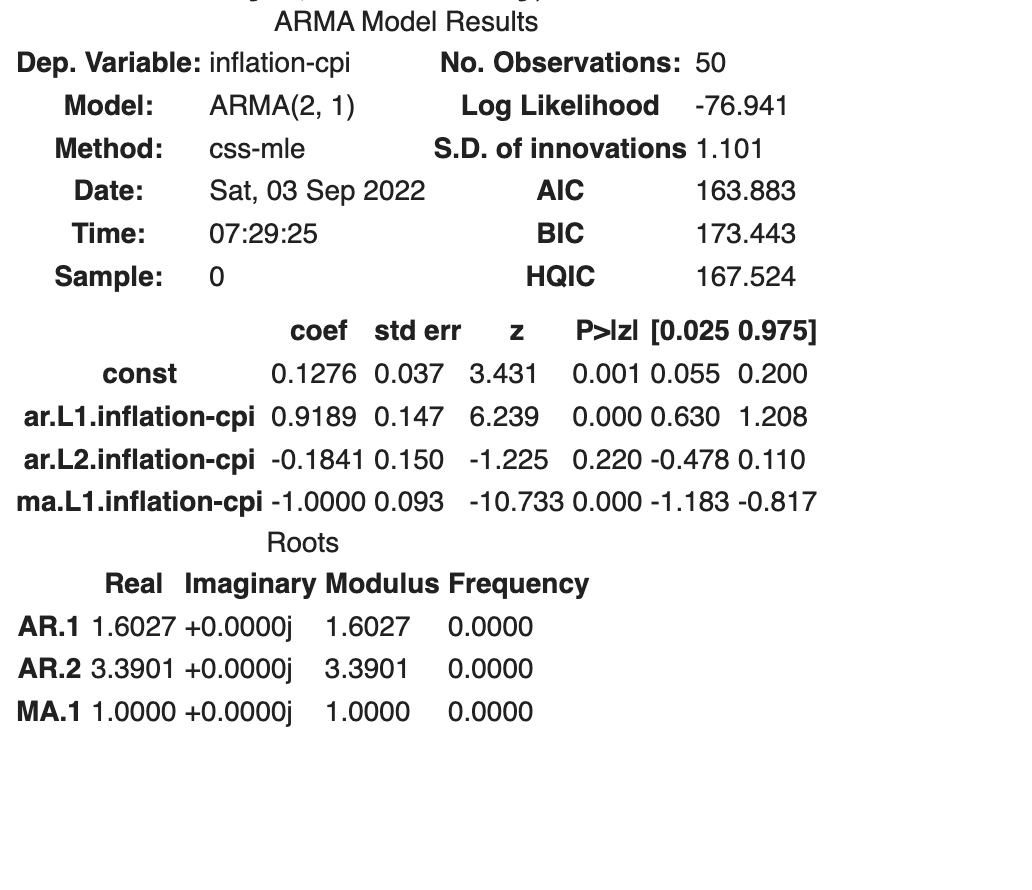
\includegraphics[width=0.7\textwidth]{Images/ARMA.png}
    \caption{Summary}
    \label{fig1}
\end{figure}

\begin{figure}[H]
    \centering
    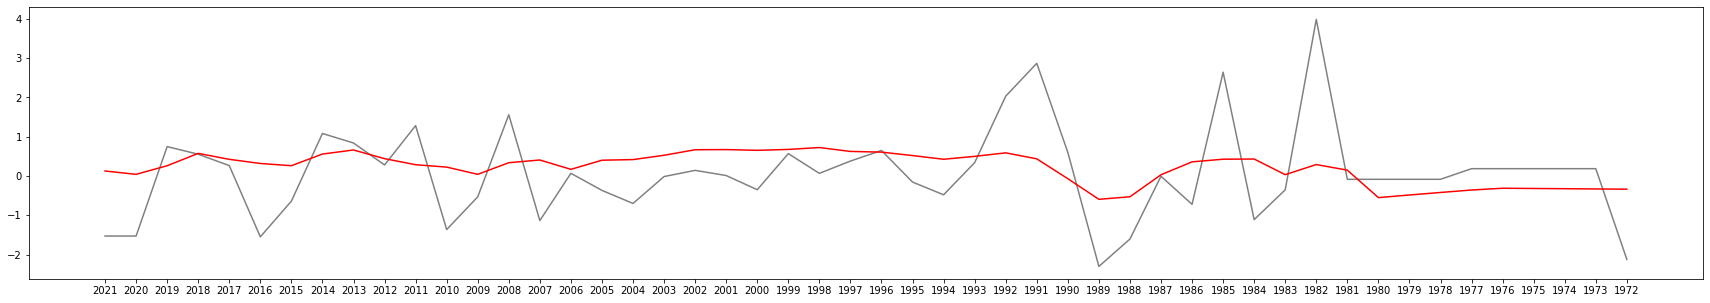
\includegraphics[width=0.7\textwidth]{Images/ARMA_P.png}
    \caption{Output Plot}
    \label{fig1}
\end{figure}

Root Mean Squared Error:  1.9255240290344706




\section{Multi-variate Model}
\subsection{VAR}
\subsubsection{Theory}
A multivariate time series model called the vector autoregressive (VAR) model connects the current observations of a variable to its historical observations as well as historical data of other variables in the system.

VAR models differ from univariate autoregressive models because they allow feedback to occur between the variables in the model. 

As an example suppose that we measure five different time series variables, denoted by $x_{t,1}$, $x_{t,2}$, $x_{t,3}$, $x_{t,4}$, $x_{t,4}$.

The vector autoregressive model of order 1, denoted as VAR(1), is as follows:

$$ x_{t,1} = \alpha_1 + \phi_{11}x_{t-1,1} + \phi_{12}x_{t-1,2} + \phi_{13}x_{t-1,3} + \phi_{14}x_{t-1,4} \phi_{15}x_{t-1,5} + \omega_{t,1}$$

$$ x_{t,2} = \alpha_2 + \phi_{21}x_{t-1,1} + \phi_{22}x_{t-1,2} + \phi_{23}x_{t-1,3} + \phi_{24}x_{t-1,4} \phi_{25}x_{t-1,5} + \omega_{t,2}$$

$$ x_{t,3} = \alpha_3 + \phi_{31}x_{t-1,1} + \phi_{32}x_{t-1,2} + \phi_{33}x_{t-1,3} + \phi_{34}x_{t-1,4} \phi_{35}x_{t-1,5} + \omega_{t,3}$$

$$ x_{t,4} = \alpha_4 + \phi_{41}x_{t-1,1} + \phi_{42}x_{t-1,2} + \phi_{43}x_{t-1,3} + \phi_{44}x_{t-1,4} \phi_{45}x_{t-1,5} + \omega_{t,4}$$

$$ x_{t,5} = \alpha_5 + \phi_{51}x_{t-1,1} + \phi_{52}x_{t-1,2} + \phi_{53}x_{t-1,3} + \phi_{54}x_{t-1,4} \phi_{55}x_{t-1,5} + \omega_{t,5}$$


Each variable is a linear function of the lag 1 values for all variables in the set.
\vspace{10mm}

Advantage of VAR Model:
\begin{itemize}
    \item A systematic but flexible approach for capturing complex real-world behavior.
\item Better forecasting performance.
\item	Ability to capture the intertwined dynamics of time series data.
\end{itemize}

\subsubsection{Python Script} 
\begin{lstlisting}[language=Python]
from statsmodels.graphics.tsaplots import plot_acf, plot_pacf
from statsmodels.tsa.statespace.varmax import VARMAX
from statsmodels.tsa.api import VAR
from statsmodels.tsa.stattools import grangercausalitytests, adfuller
from tqdm import tqdm_notebook
from itertools import product

import matplotlib.pyplot as plt
import statsmodels.api as sm
import pandas as pd
import numpy as np

import warnings
warnings.filterwarnings('ignore')

#splitting train and test data
df7 = df6
df7 = df7.set_index('tmp')
train_df=df7[12:]
test_df=df7[:12]


model = VAR(train_df.diff()[1:])
sorted_order=model.select_order(maxlags=5)
print(sorted_order.summary())

n_forecast = 12
predict = fitted_model.get_prediction(start=len(train_df),end=len(train_df) + n_forecast-1)#start="1989-07-01",end='1999-01-01')

predictions=predict.predicted_mean

predictions.columns=['gdp-p-capita-predicted','inflation-predicted', 'gdp-growth-predicted','unemp-total-predicted','p-remittances-predicted']
predictions
inf_pred = list(predictions['inflation-predicted'])
inf_ori = list(test_df['inflation-cpi'])

inf_ori_rev = inf_ori
inf_ori_rev.reverse()
plt.plot(inf_pred,color="gray")
plt.plot(inf_ori_rev,color="red")
plt.show()

from sklearn.metrics import mean_squared_error
import math 
from statistics import mean

rmse_inflation=math.sqrt(mean_squared_error(predictions['inflation-predicted'],test_df['inflation-cpi']))
print('Mean value of Inflation is : {}. Root Mean Squared Error is :{}'.format(mean(test_df['inflation-cpi']),rmse_inflation))

\end{lstlisting}

\subsubsection{Model Summary} 

\begin{figure}[H]
    \centering
    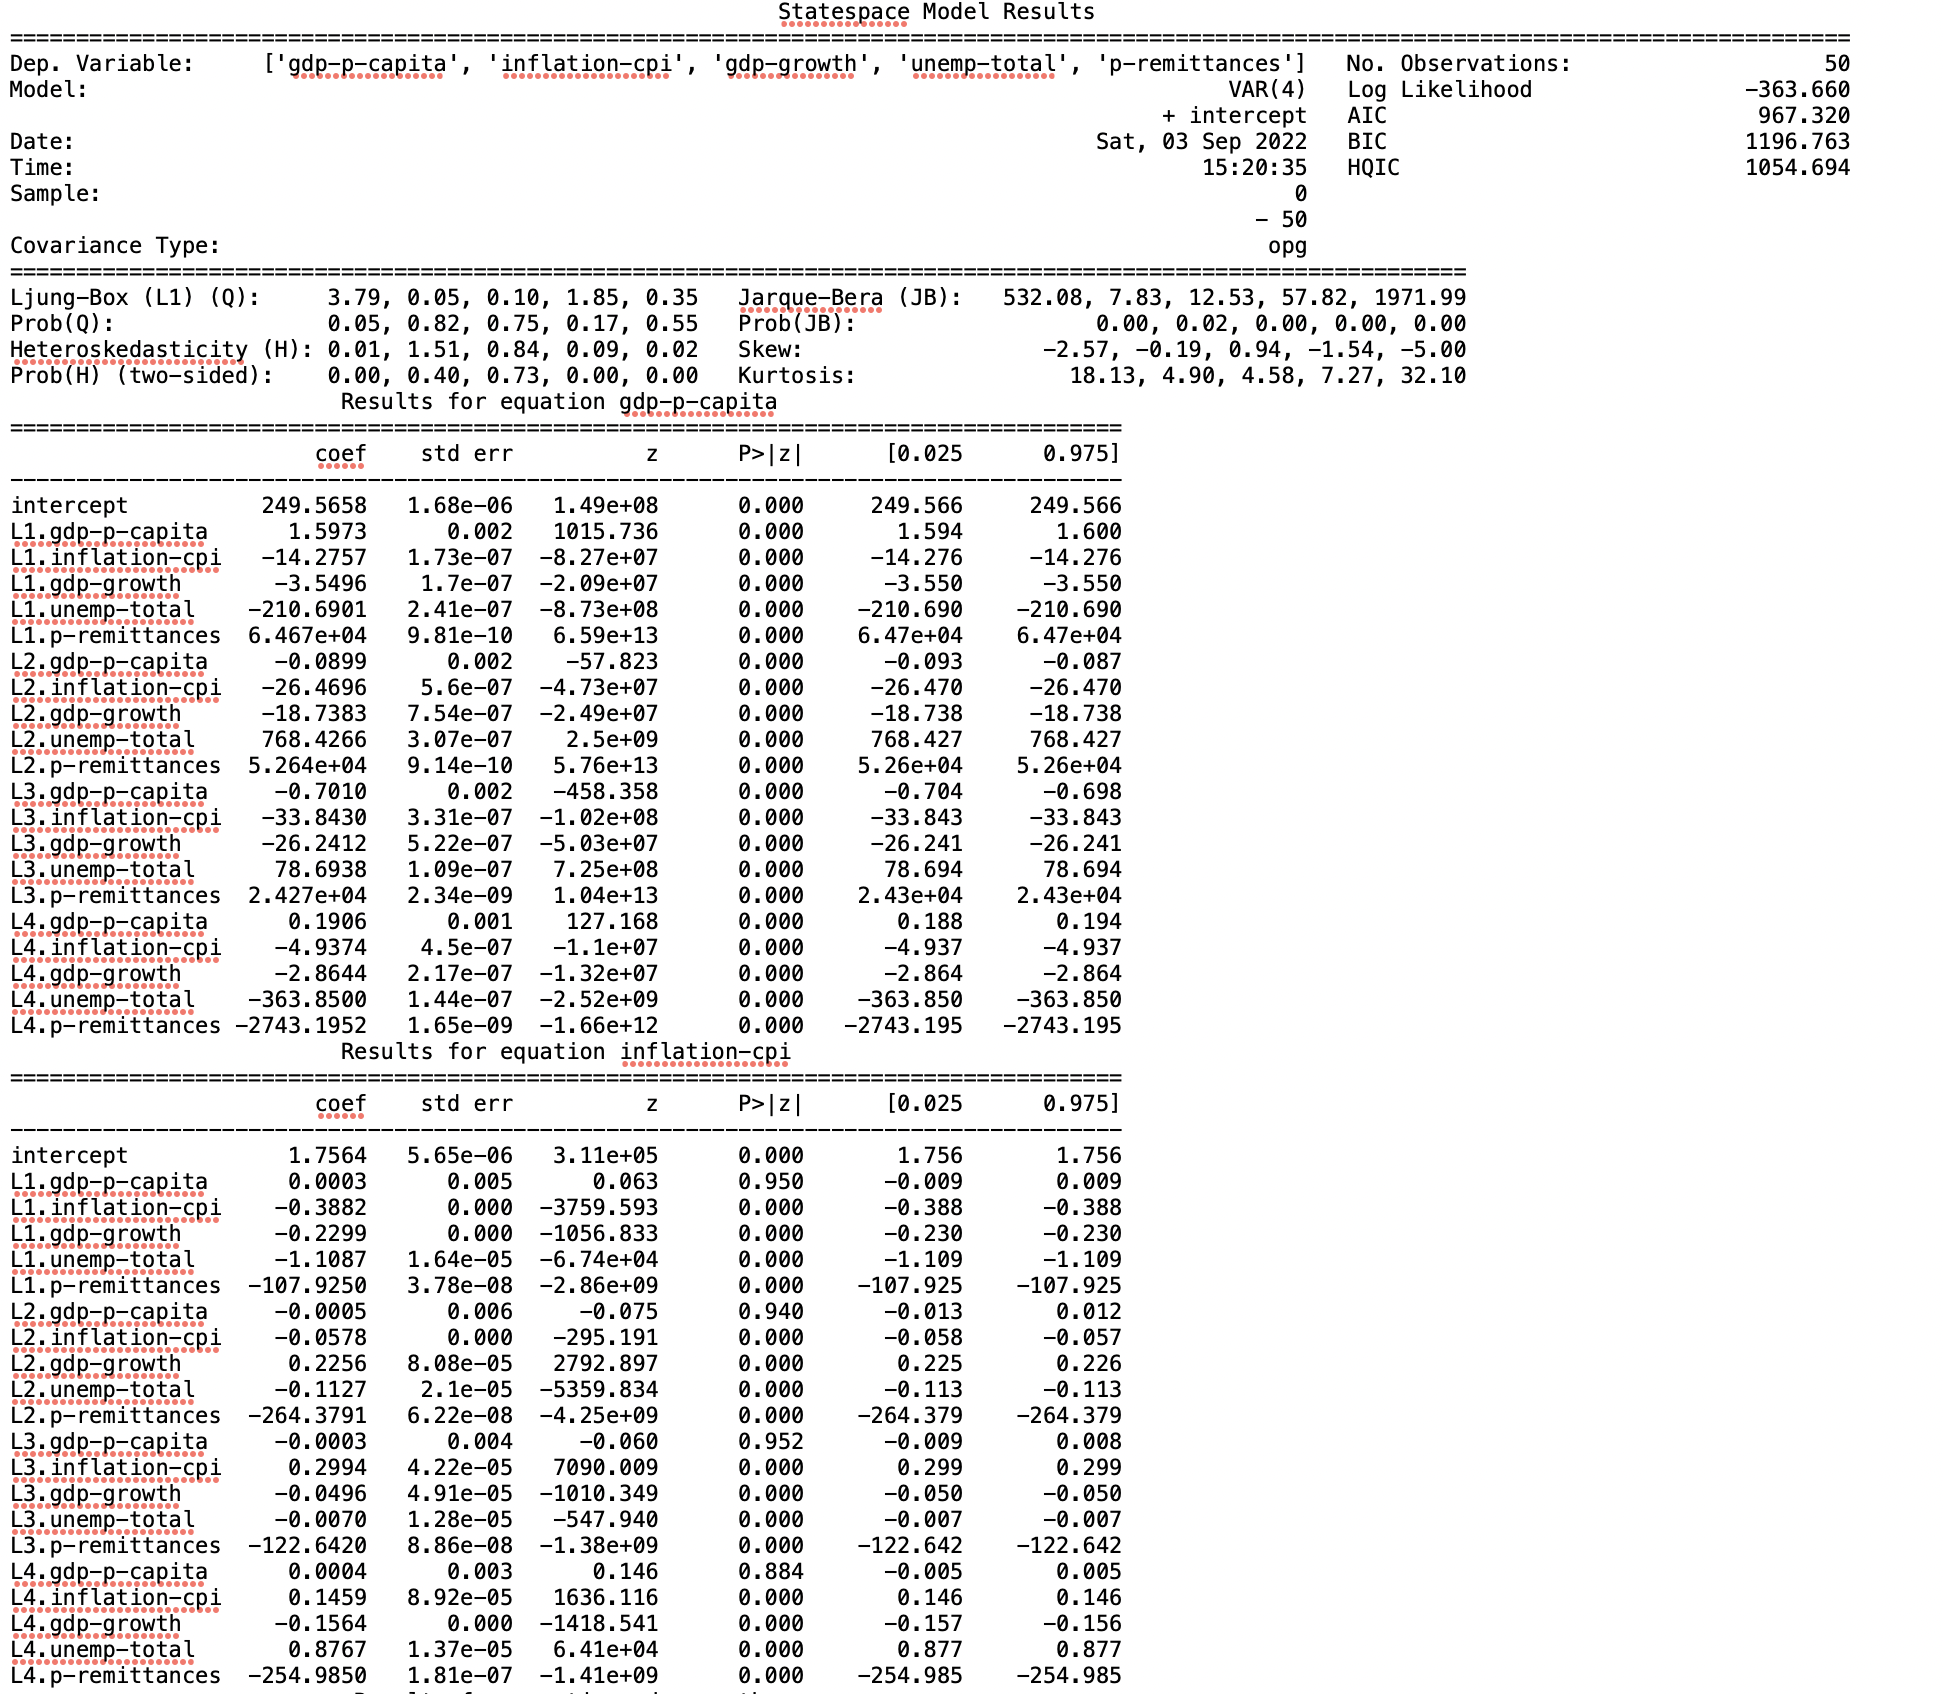
\includegraphics[width=0.7\textwidth]{Images/var1.png}
    \caption{Summary}
    \label{fig1}
\end{figure}

\begin{figure}[H]
    \centering
    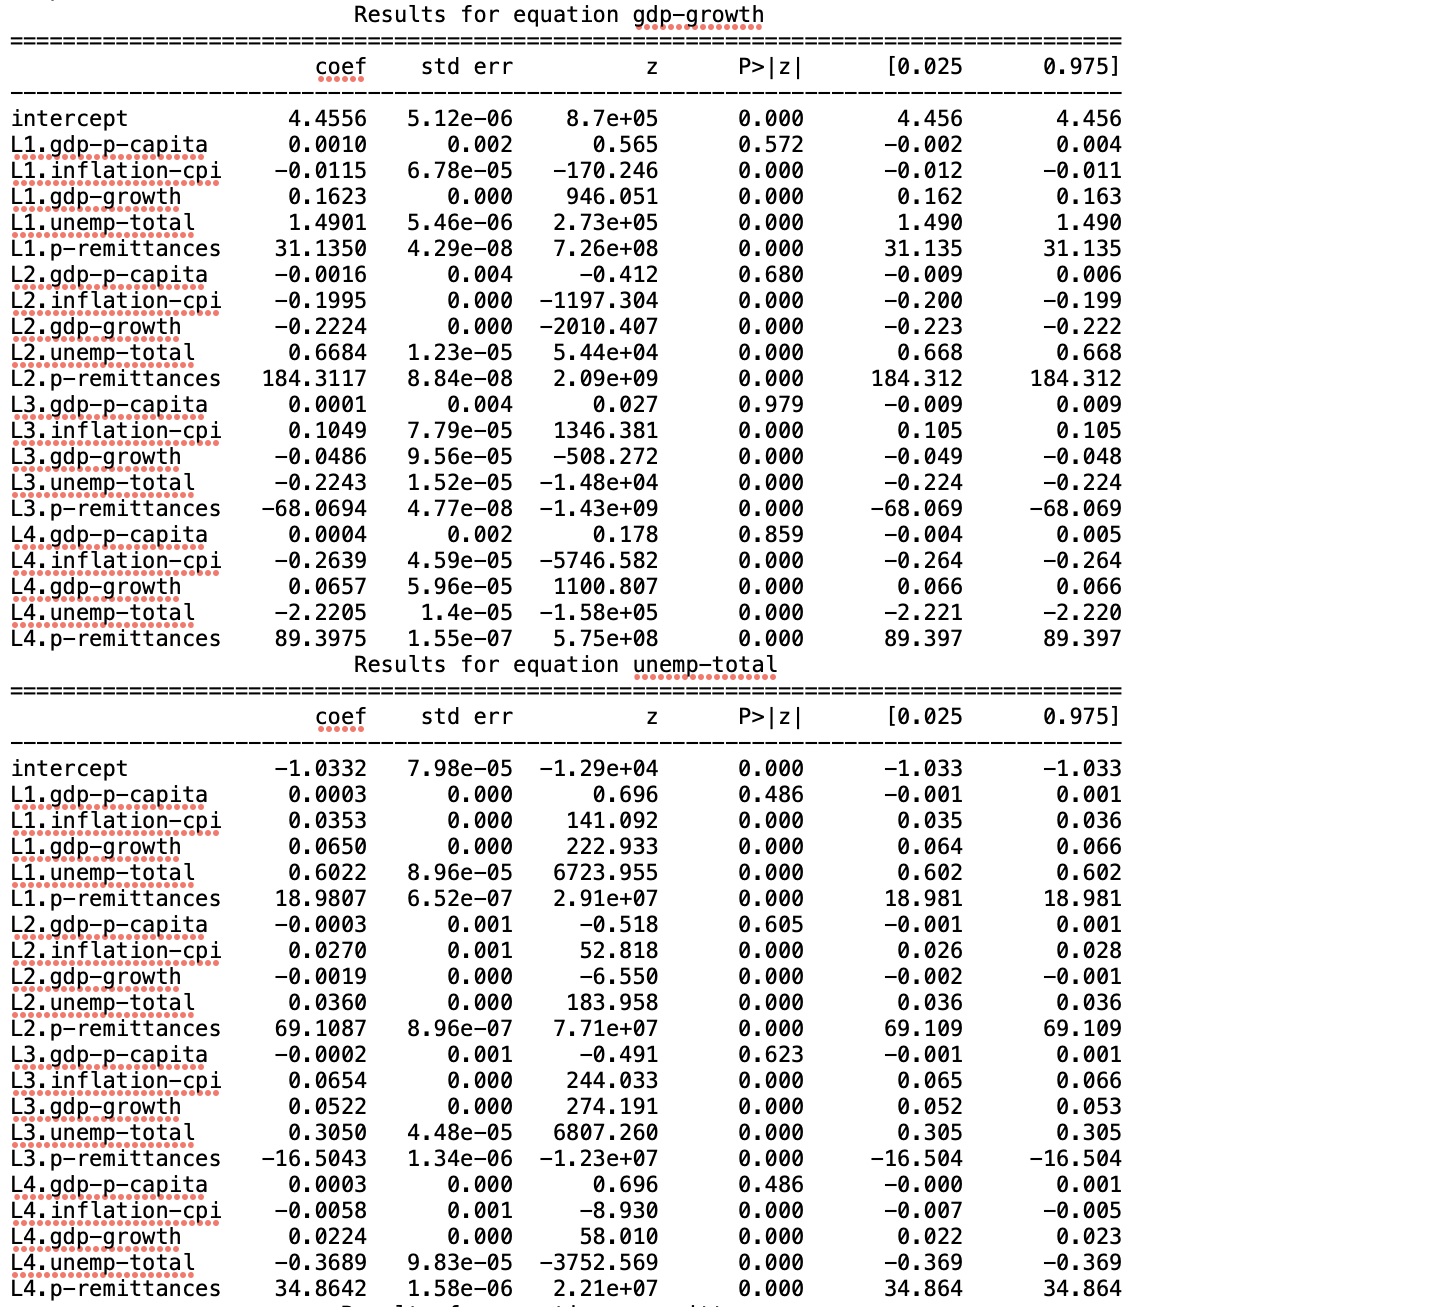
\includegraphics[width=0.7\textwidth]{Images/var2.png}
    \caption{Summary}
    \label{fig1}
\end{figure}


\begin{figure}[H]
    \centering
    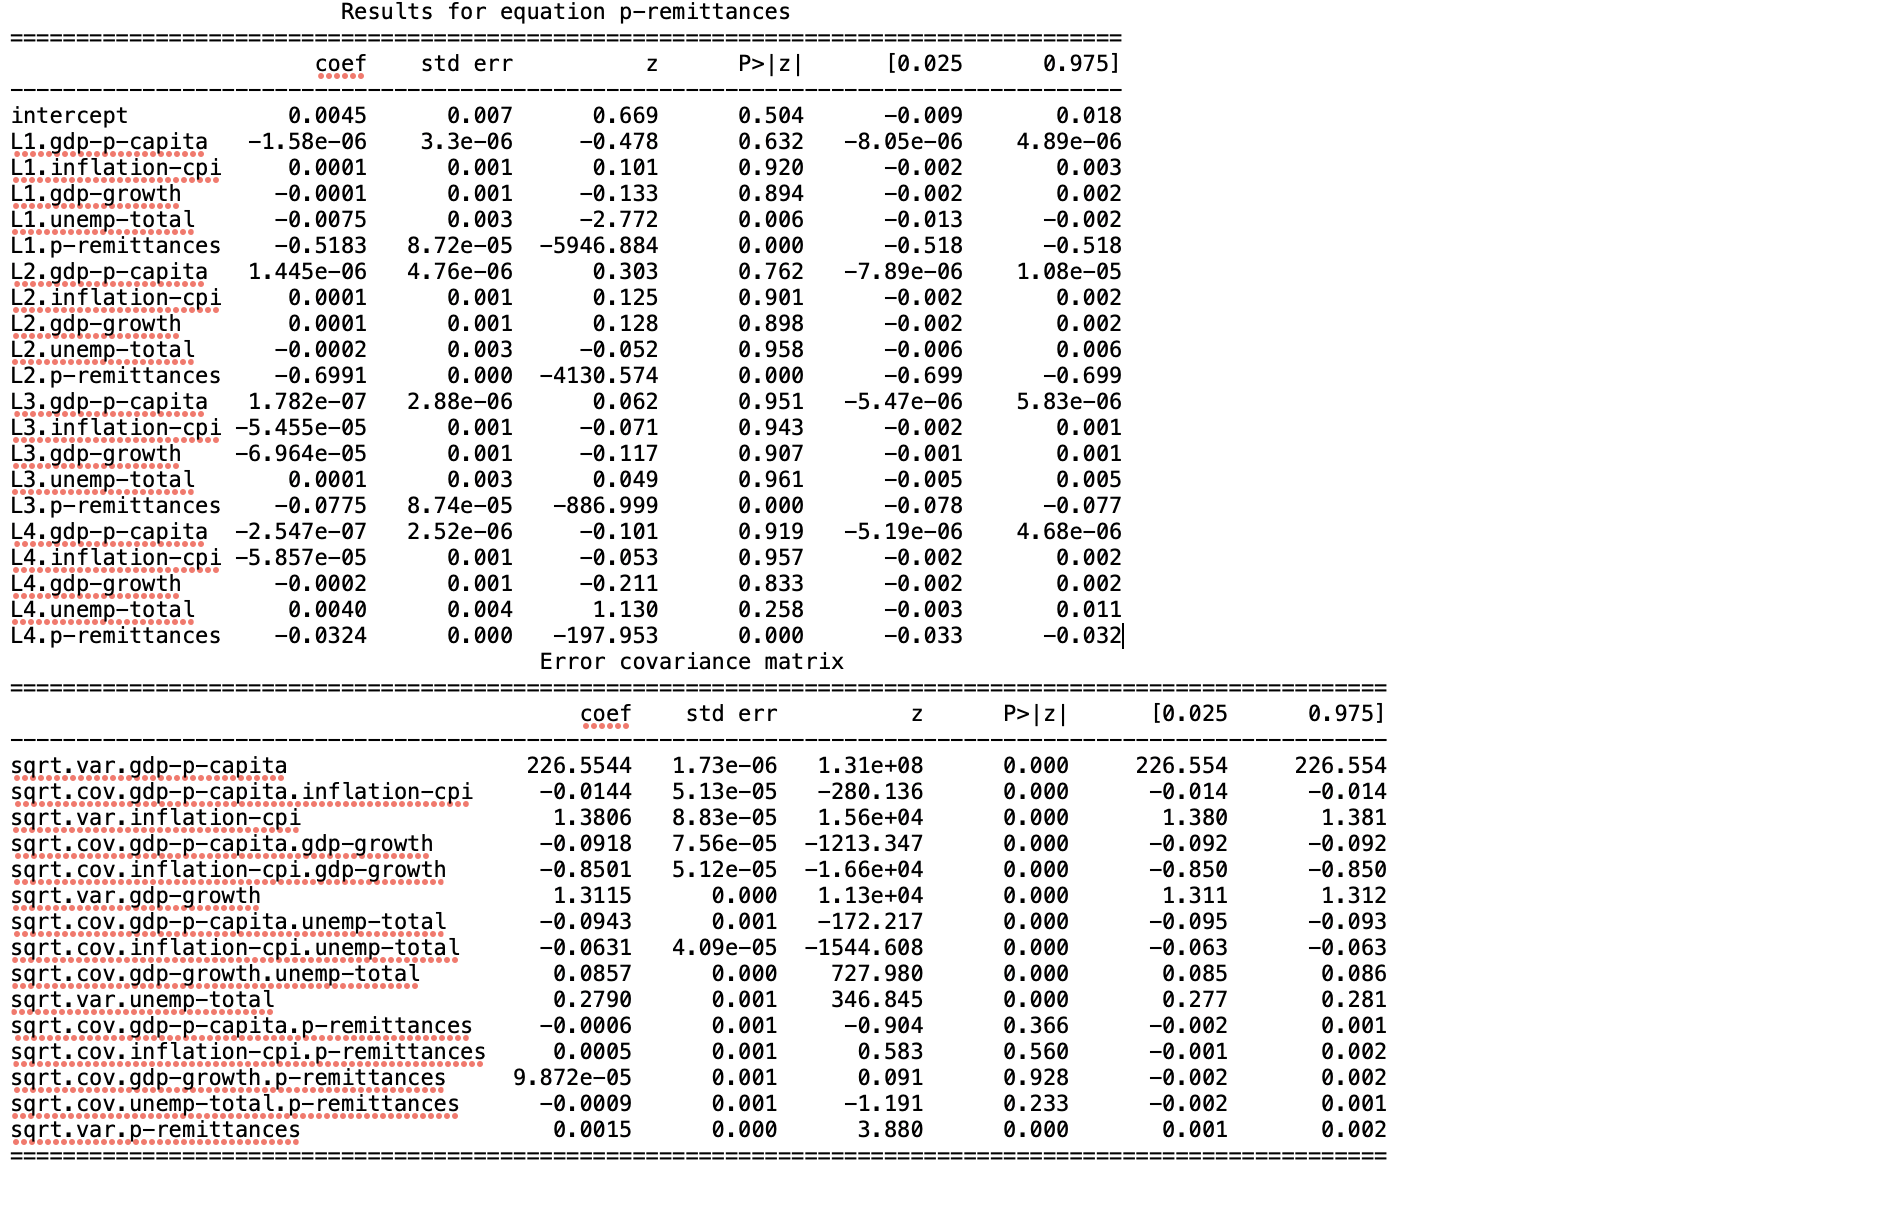
\includegraphics[width=0.7\textwidth]{Images/var3.png}
    \caption{Summary}
    \label{fig1}
\end{figure}

\begin{figure}[H]
    \centering
    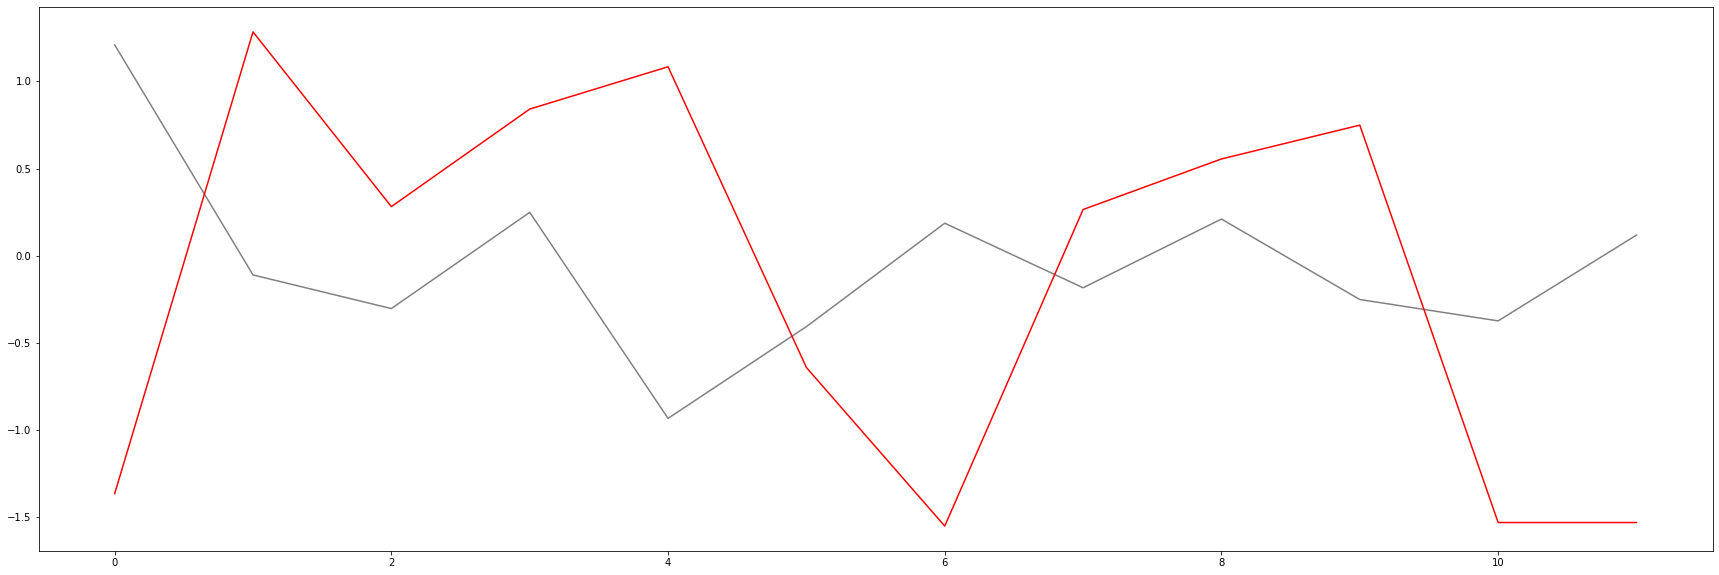
\includegraphics[width=0.7\textwidth]{Images/VAR_P.png}
    \caption{Summary}
    \label{fig1}
\end{figure}

Root Mean Squared Error is :1.3339748002157708









\subsection{LSTM Based Model}

\subsubsection{Theory}
Recurrent neural networks are a type of long short term memory. The output from the previous phase is sent into the current step of an RNN as input. Hochreiter & Schmidhuber created LSTM. It addressed the issue of long-term RNN dependency, in which the RNN can predict words from current data but cannot predict words held in long-term memory. RNN's performance becomes less effective as the gap length increases. By default, LSTM can save the data for a very long time. It is utilised for time-series data processing, forecasting, and classification.

Structure Of LSTM: \\
LSTM has a chain structure that contains four neural networks and different memory blocks called cells.

\begin{figure}[H]
    \centering
    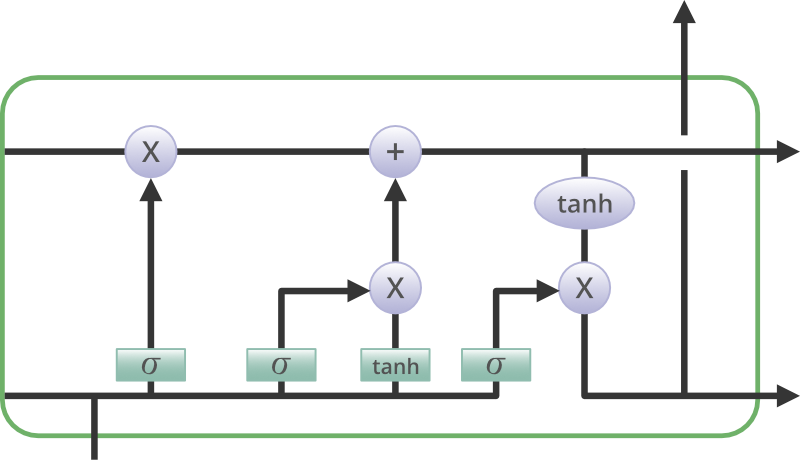
\includegraphics[width=0.7\textwidth]{Images/lstm1.png}
    \caption{LSTM Structure}
    \label{fig1}
\end{figure}

Information is retained by the cells and the memory manipulations are done by the gates. There are three gates – \\
Forget Gate: The forget gate purges the data that is no longer relevant in the cell state. The gate receives two inputs, $x_t$ (input at the current time) and $h_{t-1}$ (prior cell output), which are multiplied with weight matrices before bias is added. The output of the activation function, which receives the outcome, is binary. If a cell state's output is 0, the piece of information is lost, however if it is 1, the information is saved for use in the future.
\begin{figure}[H]
    \centering
    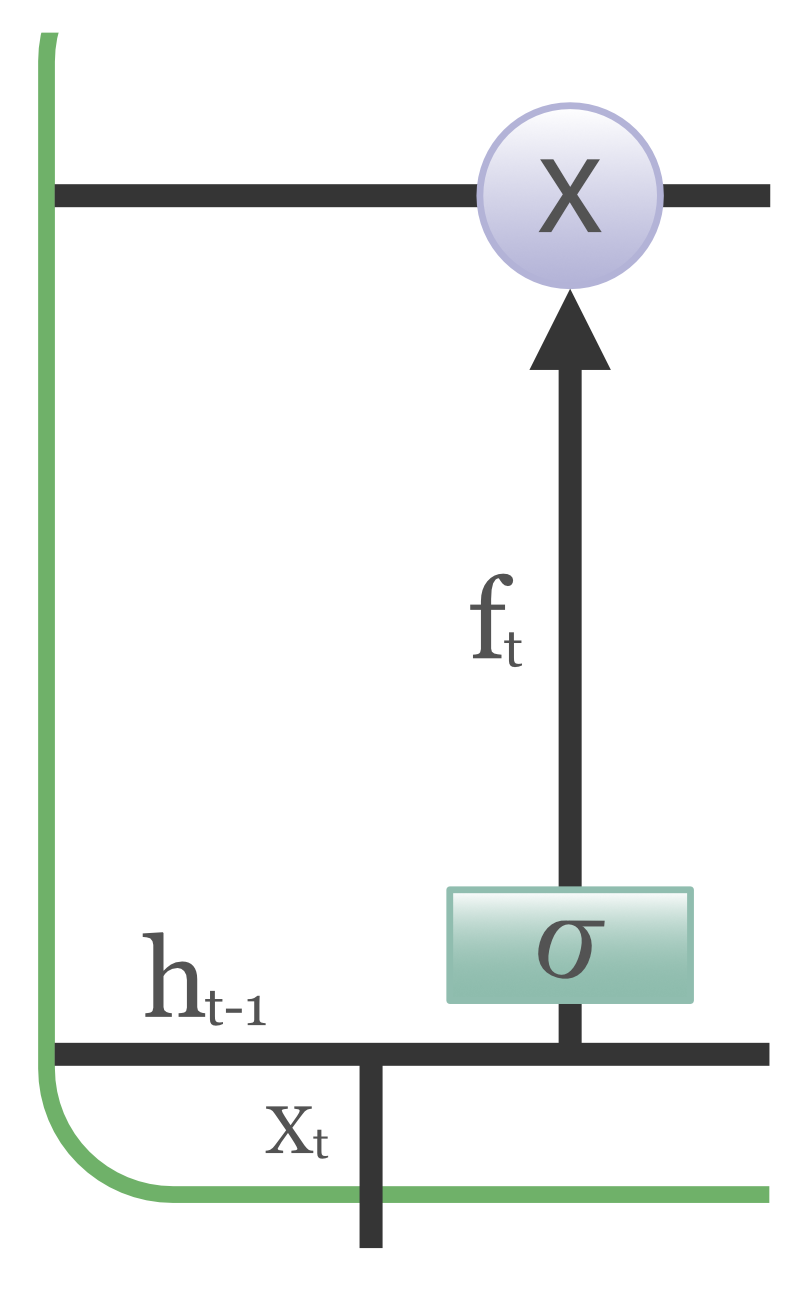
\includegraphics[width=0.7\textwidth]{Images/lstm_forget.png}
    \caption{Forget Gate}
    \label{fig1}
\end{figure}

Input Gate: The input gate updates the cell state with pertinent information. To start, the inputs $h_{t-1}$ and $x_t$ are used to regulate the information using the sigmoid function and filter the values that need to be remembered similarly to the forget gate. Then, a vector containing every possible value between $h_{t-1}$ and $x_t$ is produced using the $tanh$ function, which produces an output ranging from -1 to +1. To extract the useful information, the vector's values and the controlled values are finally multiplied.


\begin{figure}[H]
    \centering
    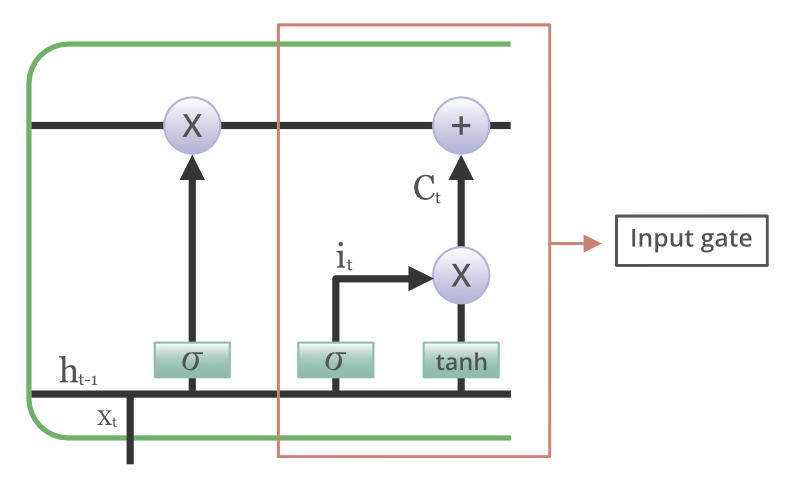
\includegraphics[width=0.7\textwidth]{Images/lstm_input.png}
    \caption{Input Gate}
    \label{fig1}
\end{figure}

Output Gate: The output gate's job is to take meaningful information out of the current cell state and deliver it as output. The $tanh$ function is first used to the cell to create a vector. The data is then filtered by the values to be remembered using the inputs $h_{t-1}$ and $x_t$, and the information is then controlled using the sigmoid function. The vector's values and the controlled values are finally multiplied and supplied as input and output to the following cell, respectively.

\begin{figure}[H]
    \centering
    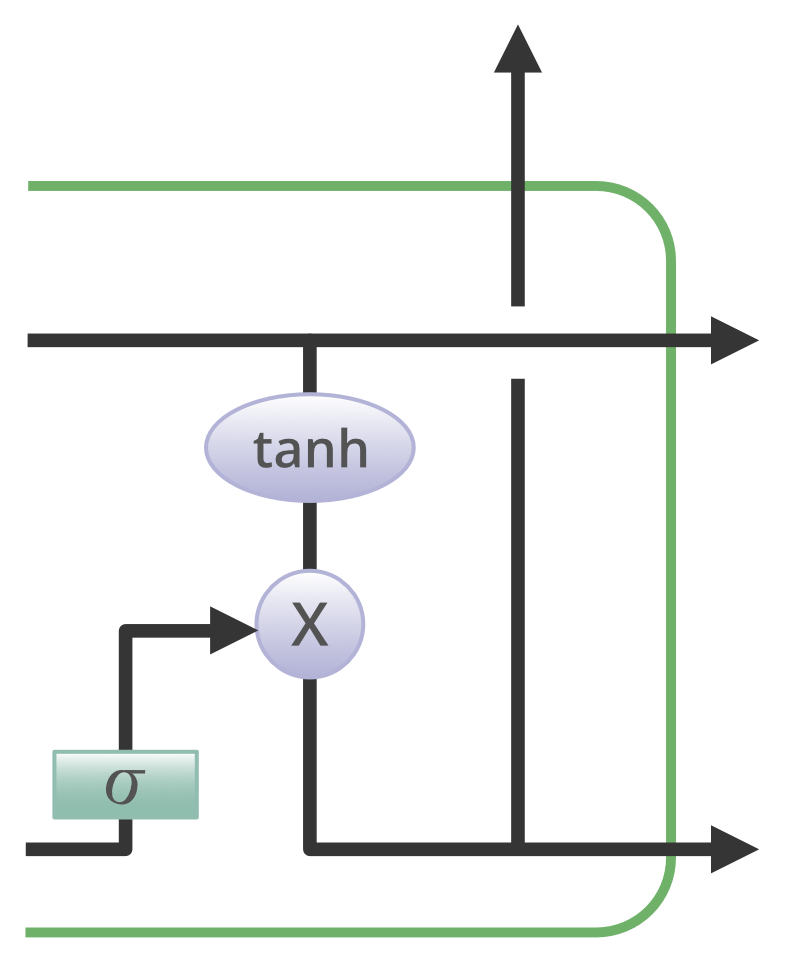
\includegraphics[width=0.7\textwidth]{Images/lstm_output.png}
    \caption{Output Gate}
    \label{fig1}
\end{figure}

\subsubsection{Python Script} 
\begin{lstlisting}[language=Python]
# import related libraries
from sklearn.preprocessing import MinMaxScaler
from sklearn.preprocessing import LabelEncoder
from sklearn.metrics import mean_squared_error
from keras.models import Sequential
from keras.layers import Dense
from keras.layers import LSTM
from sklearn.preprocessing import LabelEncoder
from sklearn.preprocessing import MinMaxScaler
import pandas as pd
import numpy as np
import seaborn as sns
from matplotlib import pyplot as plt
import math 
from pandas import DataFrame
from pandas import concat
from numpy import concatenate

def series_to_supervised(data, n_in=1, n_out=1, dropnan=True):
    n_vars = 1 if type(data) is list else data.shape[1]
    df = DataFrame(data)
    cols, names = list(), list()
    # input sequence (t-n, ... t-1)
    for i in range(n_in, 0, -1):
        cols.append(df.shift(i))
        names += [('var%d(t-%d)' % (j+1, i)) for j in range(n_vars)]
    # forecast sequence (t, t+1, ... t+n)
    for i in range(0, n_out):
        cols.append(df.shift(-i))
        if i == 0:
            names += [('var%d(t)' % (j+1)) for j in range(n_vars)]
        else:
            names += [('var%d(t+%d)' % (j+1, i)) for j in range(n_vars)]
    # put it all together
    agg = concat(cols, axis=1)
    agg.columns = names
    # drop rows with NaN values
    if dropnan:
        agg.dropna(inplace=True)
    return agg

    # normalize features
scaler = MinMaxScaler(feature_range=(0, 1))
scaled = scaler.fit_transform(df7)

# frame as supervised learning
reframed = series_to_supervised(scaled, 1, 1)

a = range(20,10,1)
reframed.drop(reframed.columns[a], axis=1, inplace=True)
reframed.dtypes

values = reframed.values
train = values[12:, :]
test = values[:12]
# split into input and outputs
train_X, train_y = train[:, :-1], train[:, -4]
test_X, test_y = test[:, :-1], test[:, -4]
# reshape input to be 3D [samples, timesteps, features]
train_X = train_X.reshape((train_X.shape[0], 1, train_X.shape[1]))
test_X = test_X.reshape((test_X.shape[0], 1, test_X.shape[1]))
print(train_X.shape, train_y.shape, test_X.shape, test_y.shape)

model = Sequential()
model.add(LSTM(50, input_shape=(train_X.shape[1], train_X.shape[2])))
model.add(Dense(1))
model.compile(loss='mae', optimizer='adam')
# fit network
history = model.fit(train_X, train_y, epochs=50, batch_size=72, validation_data=(test_X, test_y), verbose=2, shuffle=False)
# plot history
plt.plot(history.history['loss'], label='train')
plt.plot(history.history['val_loss'], label='test')
plt.legend()
plt.show()

#make a prediction
yhat = model.predict(test_X)
test_X = test_X.reshape((test_X.shape[0], test_X.shape[2]))
# invert scaling for forecast
inv_yhat = concatenate((yhat, test_X[:, 1:]), axis=1)
scaled = scaler.fit_transform(test_X)
inv_yhat = scaler.inverse_transform(inv_yhat)
inv_yhat = inv_yhat[:,0]
# invert scaling for actual
test_y = test_y.reshape((len(test_y), 1))
inv_y = concatenate((test_y, test_X[:, 1:]), axis=1)
inv_y = scaler.inverse_transform(inv_y)
inv_y = inv_y[:,0]
# calculate RMSE
rmse = math.sqrt(mean_squared_error(inv_y, inv_yhat))
print('Test RMSE: %.3f' % rmse)

#Ploting Fitted and Actual values
plt.plot(inv_y,color="gray")
plt.plot(inv_yhat,color="red")
plt.show()


\end{lstlisting}


\subsubsection{Model Summary} 

Epoch 1/50 \\
1/1 - 3s - loss: 0.4748 - val\_loss: 0.2503 - 3s/epoch - 3s/step \\
Epoch 2/50 \\
1/1 - 0s - loss: 0.4598 - val\_loss: 0.2282 - 37ms/epoch - 37ms/step \\
Epoch 3/50 \\
1/1 - 0s - loss: 0.4447 - val\_loss: 0.2061 - 41ms/epoch - 41ms/step \\
Epoch 4/50 \\
1/1 - 0s - loss: 0.4295 - val\_loss: 0.1838 - 40ms/epoch - 40ms/step \\
Epoch 5/50 \\
1/1 - 0s - loss: 0.4143 - val\_loss: 0.1614 - 35ms/epoch - 35ms/step \\
Epoch 6/50 \\
1/1 - 0s - loss: 0.3990 - val\_loss: 0.1388 - 56ms/epoch - 56ms/step \\
Epoch 7/50 \\
1/1 - 0s - loss: 0.3836 - val\_loss: 0.1160 - 41ms/epoch - 41ms/step \\
Epoch 8/50 \\
1/1 - 0s - loss: 0.3683 - val\_loss: 0.0965 - 50ms/epoch - 50ms/step \\
Epoch 9/50 \\
1/1 - 0s - loss: 0.3535 - val\_loss: 0.0806 - 43ms/epoch - 43ms/step \\
Epoch 10/50 \\
1/1 - 0s - loss: 0.3391 - val\_loss: 0.0688 - 36ms/epoch - 36ms/step \\
Epoch 11/50 \\
1/1 - 0s - loss: 0.3248 - val\_loss: 0.0586 - 38ms/epoch - 38ms/step \\
Epoch 12/50 \\
1/1 - 0s - loss: 0.3105 - val\_loss: 0.0584 - 42ms/epoch - 42ms/step \\
Epoch 13/50 \\
1/1 - 0s - loss: 0.2961 - val\_loss: 0.0643 - 36ms/epoch - 36ms/step \\
Epoch 14/50 \\
1/1 - 0s - loss: 0.2815 - val\_loss: 0.0746 - 34ms/epoch - 34ms/step \\
Epoch 15/50 \\
1/1 - 0s - loss: 0.2669 - val\_loss: 0.0909 - 34ms/epoch - 34ms/step \\
Epoch 16/50 \\
1/1 - 0s - loss: 0.2521 - val\_loss: 0.1075 - 39ms/epoch - 39ms/step \\
Epoch 17/50 \\
1/1 - 0s - loss: 0.2371 - val\_loss: 0.1271 - 37ms/epoch - 37ms/step \\
Epoch 18/50 \\
1/1 - 0s - loss: 0.2232 - val\_loss: 0.1480 - 61ms/epoch - 61ms/step \\
Epoch 19/50 \\
1/1 - 0s - loss: 0.2110 - val\_loss: 0.1725 - 38ms/epoch - 38ms/step \\
Epoch 20/50 \\
1/1 - 0s - loss: 0.2000 - val\_loss: 0.1973 - 35ms/epoch - 35ms/step \\
Epoch 21/50 \\
1/1 - 0s - loss: 0.1920 - val\_loss: 0.2206 - 35ms/epoch - 35ms/step \\
Epoch 22/50 \\
1/1 - 0s - loss: 0.1868 - val\_loss: 0.2422 - 35ms/epoch - 35ms/step \\
Epoch 23/50 \\
1/1 - 0s - loss: 0.1838 - val\_loss: 0.2620 - 33ms/epoch - 33ms/step \\
Epoch 24/50 \\
1/1 - 0s - loss: 0.1810 - val\_loss: 0.2798 - 39ms/epoch - 39ms/step \\
Epoch 25/50 \\
1/1 - 0s - loss: 0.1795 - val\_loss: 0.2953 - 35ms/epoch - 35ms/step \\
Epoch 26/50 \\
1/1 - 0s - loss: 0.1789 - val\_loss: 0.3085 - 44ms/epoch - 44ms/step \\
Epoch 27/50 \\
1/1 - 0s - loss: 0.1789 - val\_loss: 0.3196 - 38ms/epoch - 38ms/step \\
Epoch 28/50 \\
1/1 - 0s - loss: 0.1790 - val\_loss: 0.3286 - 35ms/epoch - 35ms/step \\
Epoch 29/50 \\
1/1 - 0s - loss: 0.1793 - val\_loss: 0.3354 - 34ms/epoch - 34ms/step \\
Epoch 30/50 \\
1/1 - 0s - loss: 0.1797 - val\_loss: 0.3404 - 35ms/epoch - 35ms/step \\
Epoch 31/50 \\
1/1 - 0s - loss: 0.1798 - val\_loss: 0.3435 - 36ms/epoch - 36ms/step \\
Epoch 32/50 \\
1/1 - 0s - loss: 0.1797 - val\_loss: 0.3451 - 45ms/epoch - 45ms/step \\
Epoch 33/50 \\
1/1 - 0s - loss: 0.1795 - val\_loss: 0.3450 - 38ms/epoch - 38ms/step \\
Epoch 34/50 \\
1/1 - 0s - loss: 0.1791 - val\_loss: 0.3432 - 33ms/epoch - 33ms/step \\ 
Epoch 35/50 \\
1/1 - 0s - loss: 0.1787 - val\_loss: 0.3398 - 38ms/epoch - 38ms/step \\
Epoch 36/50 \\
1/1 - 0s - loss: 0.1779 - val\_loss: 0.3350 - 40ms/epoch - 40ms/step \\
Epoch 37/50 \\
1/1 - 0s - loss: 0.1770 - val\_loss: 0.3288 - 39ms/epoch - 39ms/step \\
Epoch 38/50 \\
1/1 - 0s - loss: 0.1758 - val\_loss: 0.3215 - 35ms/epoch - 35ms/step \\
Epoch 39/50 \\
1/1 - 0s - loss: 0.1745 - val\_loss: 0.3134 - 41ms/epoch - 41ms/step \\
Epoch 40/50 \\
1/1 - 0s - loss: 0.1731 - val\_loss: 0.3048 - 40ms/epoch - 40ms/step \\
Epoch 41/50 \\
1/1 - 0s - loss: 0.1716 - val\_loss: 0.2957 - 36ms/epoch - 36ms/step \\
Epoch 42/50 \\
1/1 - 0s - loss: 0.1702 - val\_loss: 0.2863 - 39ms/epoch - 39ms/step \\
Epoch 43/50 \\
1/1 - 0s - loss: 0.1687 - val\_loss: 0.2767 - 45ms/epoch - 45ms/step \\
Epoch 44/50 \\
1/1 - 0s - loss: 0.1672 - val\_loss: 0.2669 - 40ms/epoch - 40ms/step \\
Epoch 45/50 \\
1/1 - 0s - loss: 0.1657 - val\_loss: 0.2569 - 41ms/epoch - 41ms/step \\
Epoch 46/50 \\
1/1 - 0s - loss: 0.1642 - val\_loss: 0.2468 - 38ms/epoch - 38ms/step \\
Epoch 47/50 \\
1/1 - 0s - loss: 0.1627 - val\_loss: 0.2366 - 60ms/epoch - 60ms/step \\
Epoch 48/50 \\
1/1 - 0s - loss: 0.1611 - val\_loss: 0.2263 - 41ms/epoch - 41ms/step \\
Epoch 49/50 \\
1/1 - 0s - loss: 0.1596 - val\_loss: 0.2159 - 41ms/epoch - 41ms/step \\
Epoch 50/50 \\
1/1 - 0s - loss: 0.1580 - val\_loss: 0.2055 - 38ms/epoch - 38ms/step \\

\begin{figure}[H]
    \centering
    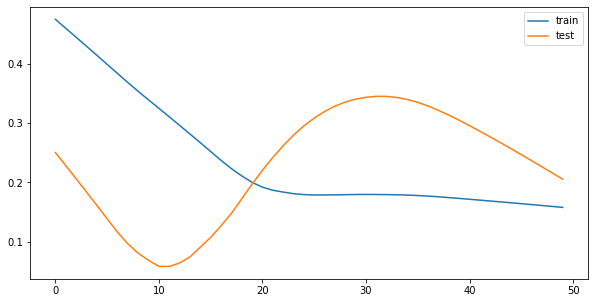
\includegraphics[width=0.7\textwidth]{Images/LSTM_L.png}
    \caption{Loss Plot}
    \label{fig1}
\end{figure}

\begin{figure}[H]
    \centering
    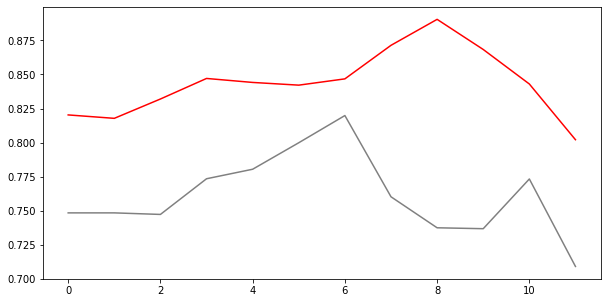
\includegraphics[width=0.7\textwidth]{Images/LSTM_P.png}
    \caption{Output Plot}
    \label{fig1}
\end{figure}

Root Mean Squared Error: 0.089



